\chapter{گزارش}

\section{مسئله}
	
در این پروژه قصد داشتیم تا پارامترهای مدل کانال در
\lr{Large-scale}
 را در یک سامانه مخابرات بی‌سیم تخمین بزنیم. 

در مدل یک کانال محوشدگی از دیدگاه 
\lr{Large-scale}، 
دو عامل افت مسیر و سایه‌شدگی نقش اساسی را ایفا می‌کردند. می‌دانیم که کانال را در حضور این دو عامل میتوان به صورت زیر مدل نمود:
\begin{figure}[H]
	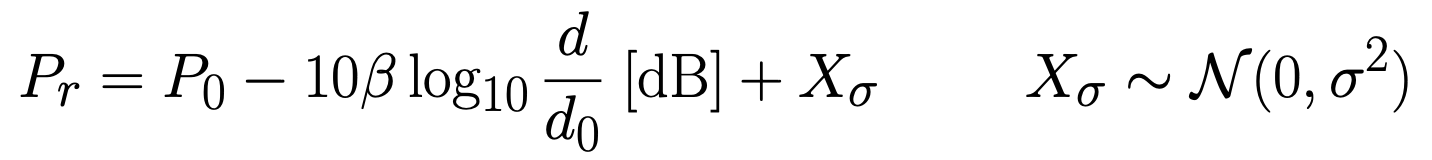
\includegraphics[width=0.75\columnwidth]{Picture/formula.png}
	\centering
\end{figure}
در این پروژه نیز تلاش شد راه حلی ارائه شود تا این این دو عامل تخمین زده شوند.

ما در این پروژه با داده‌های تست درایو در یک شبکه سلولی مواجه بودیم که شامل قدرت سیگنال دریافتی (به همراه موقعیت جغرافیایی هر اندازه‌گیری) بود. هدف ما این بود که پارامترهای مربوط به مدل افت مسیر، شامل توان
\lr{(\lr{P\textsubscript{0}})}، 
ضریب افت مسیر 
\lr{(\lr{$\beta$})}
و انحراف استاندارد نویز گاوسی 
\lr{(\lr{$\sigma$})}
 را تخمین بزنیم.
	
\section{راه حل}

ابتدا نرم‌افزاری در بستر اندروید پیاده‌سازی کردیم که از طریق آن توان دریافتی تلفن همراه و اطلاعات موقعیت مکانی آن را جمع‌آوری کند و پایگاه داده‌ای از این اطلاعات جمع آوری کردیم.

سپس به سراغ تخمین پارامترهای مجهول در فرمول رفتیم. ما با یک معادله‌ی خطی رو به رو بودیم که 
\lr{P\textsubscript{r}}
همان 
\lr{Y}،
\lr{10log\textsubscript{10}(d / d\textsubscript{0})}
همان
\lr{X}،
\lr{$\beta$}
همان شیب خط و 
\lr{P\textsubscript{0}}
هم عرض از مبدا آن بود.

برای حل این مسئله، ما از روش رگرسیون خطی استفاده کردیم تا بهترین خطی که بر داده‌هایی که جمع‌آوری شده، متناسب می‌شود را پیدا کنیم و متغیرهایمان را از این خط استخراج کنیم.

برای پیدا کردن 
\lr{$\sigma$}
نویز هم از اختلاف خط به دست آمده از رگرسیون خطی و خط به دست آمده از جمع‌آوری داده‌ها استفاده کردیم.

\section{توضیح کد}
	
کد پروژه از دو بخش تشکیل شده است. نرم‌افزار اندرویدی با زبان کاتلین توسعه داده‌ شده و پیدا کردن متغیرها در زبان پایتون پیاده‌سازی شده است. 
\subsection{بخش اندروید}
برنامه اندرویدی توسط زبان \lr{Kotlin} نوشته شده و به منظور جمع آوری داده های توان سیگنال و لکیشن استفاده می شود. این برنامه را می‌توان به سه بخش اصلی تقسیم کرد:
\begin{itemize}
	\item ‌صفحه اصلی: کنترل کل عملیات‌های \lr{UI} و دریافت داده
	\item کنترلر پایگاه داده: وظیفه ایجاد پایگاه داده برای برنامه، ثبت داده‌ی جدید و خروجی گرفتن از پایگاه داده در حافظه دستگاه
	\item مدل پایگاه داده: تعریف مدل استفاده شده برای وارد کردن داده در پایگاه داده
\end{itemize}

\subsubsection{صفحه اصلی}
در ابتدای اجرای برنامه و در صفحه اصلی لازم است که درخواست تایید دسترسی های لازم از کاربر پرسیده شود. به این منظور تابع بررسی دسترسی ها تعریف شده است که در صورت عدم وجود دسترسی، تاییدیه از کاربر گرفته شود.
\begin{lstlisting}[language=Java]
	@RequiresApi(Build.VERSION_CODES.Q)
	private fun checkPermissionsAndStartGatheringData() {
		// Check permissions
		if (ContextCompat.checkSelfPermission(
		this,
		Manifest.permission.ACCESS_FINE_LOCATION
		) != PackageManager.PERMISSION_GRANTED
		|| ContextCompat.checkSelfPermission(
		this,
		Manifest.permission.ACCESS_COARSE_LOCATION
		) != PackageManager.PERMISSION_GRANTED
		|| ContextCompat.checkSelfPermission(
		this,
		Manifest.permission.READ_PHONE_STATE
		) != PackageManager.PERMISSION_GRANTED
		|| ContextCompat.checkSelfPermission(
		this,
		Manifest.permission.WRITE_EXTERNAL_STORAGE
		) != PackageManager.PERMISSION_GRANTED
		) {
			// Request permissions
			ActivityCompat.requestPermissions(
			this,
			arrayOf(
			Manifest.permission.ACCESS_FINE_LOCATION,
			Manifest.permission.ACCESS_COARSE_LOCATION,
			Manifest.permission.READ_PHONE_STATE,
			Manifest.permission.WRITE_EXTERNAL_STORAGE
			),
			PERMISSION_REQUEST_CODE
			)
		}
		
		if (ContextCompat.checkSelfPermission(
		this,
		Manifest.permission.ACCESS_BACKGROUND_LOCATION
		) != PackageManager.PERMISSION_GRANTED) {
			ActivityCompat.requestPermissions(
			this,
			arrayOf(
			Manifest.permission.ACCESS_BACKGROUND_LOCATION
			),
			PERMISSION_REQUEST_CODE
			)
		} else {
			startGatheringData()
		}
	}
\end{lstlisting}

در این صفحه برای توجه به تغییرات توان سیگنال و مکان، دو \lr{listener} تعریف شده است. نحوه ی عملکرد آن ها به این صورت است که با تغییر توان سیگنال یا مکان،‌ تابع متناظر صدا زده می شود و علاوه بر تغییر \lr{UI} به جهت نمایش داده به دست آمده، تابع متناظر افزودن به پایگاه داده نیز صدا زده می شود تا داده ها وارد پایگاه داده شوند.

همچنین لازم به ذکر است که برای خواندن اطلاعات سیگنال از کتاب خانه‌ی \lr{telephony manager} استفاده شده است و برای دسترسی به مکان سیستم \lr{gms google} به کار رفته است.

\begin{lstlisting}[language=Java]
	private val signalStrengthListener = object : PhoneStateListener() {
		@SuppressLint("SetTextI18n")
		@RequiresApi(Build.VERSION_CODES.Q)
		override fun onSignalStrengthsChanged(signalStrength: SignalStrength) {
			// Handle signal strength changes here
			strength = signalStrength.cellSignalStrengths[0].dbm // Example: GSM signal strength
			signalStrengthTextView.text = "Signal Strength: $strength"
			
			addToDb()
		}
	}
	
	telephonyManager = getSystemService(Context.TELEPHONY_SERVICE) as TelephonyManager
	fusedLocationClient = LocationServices.getFusedLocationProviderClient(this)
	createLocationRequest()
	locationCallback = object : LocationCallback() {
		@SuppressLint("SetTextI18n")
		override fun onLocationResult(locationResult: LocationResult) {
			locationResult?.let {
				for (location in locationResult.locations) {
					latitude    =  String.format("%.4f", location.latitude).toDouble()
					longitude   = String.format("%.4f", location.longitude).toDouble()
					locationTextView.text = "Location: $latitude, $longitude"
					rowCountTextView.text = "Rows: $rowNumber"
					
					addToDb()
				}
			}
		}
	}
\end{lstlisting}

در صورت رخ دادن تغییر در هر یک از داده‌های توان سیگنال و مکان دستگاه، تابع افزودن اطلاعات به پایگاه داده مورد استفاده قرار می‌گیرد، در این تابع ابتدا بررسی می‌شود که هیچ یک از پارامترها مقدار صفر نداشته باشند، زیرا داده‌ی خطا محسوب می‌شوند. سپس مدل داده‌ی تعریف شده مورد استفاده قرار می‌گیرد و داده‌ها وارد پایگاه داده خواهند شد.

\begin{lstlisting}[language=Java]
	private fun addToDb() {
		val rsrp = strength
		val lat = latitude
		val lon = longitude
		
		if (rsrp != 0 && lat != 0.0 && lon != 0.0) {
			val std = DataModel(rsrp = rsrp, latitude = lat, longitude = lon)
			val status = dbHelper.insertData(std)
			
			rowNumber += 1
			//Check insert success
			if (status > -1) {
				println("Data added successfully")
			}
		}
	}
\end{lstlisting}

برای شروع کار سیستم یک دکمه در نظر گرفته شده است که وظیفه‌ی راه اندازی \lr{listener}ها مذکور را داشته و تغییرات \lr{UI} مربوطه را اعمال می کند. همچنین دکمه‌ی مذکور وظیفه ی متوقف کردن سیستم پس از راه اندازی را نیز بر عهده دارد. پس از متوقف کردن \lr{listener}های تعریف شده، سعی بر خروجی گرفتن از پایگاه داده ذخیره شده‌ی درون برنامه‌ای می‌شود. در صورت موفقیت آمیز بودن خروجی پایگاه داده فرآیند اجرای کد پایتون در برنامه صدا زده می‌شود.

\begin{lstlisting}[language=Java]
	private fun startGatheringData() {
		dbHelper = DatabaseHelper(this)
		
		// Start gathering signal power data
		telephonyManager.listen(signalStrengthListener, PhoneStateListener.LISTEN_SIGNAL_STRENGTHS)
		fusedLocationClient.requestLocationUpdates(locationRequest, locationCallback, null)
		
		isGatheringData = true
		startStopButton.text = "Stop"
		statusTextView.text = "Status: Gathering data..."
		resultsTextView.text = "No results available yet"
	}
	private fun stopGatheringData() {
		telephonyManager.listen(signalStrengthListener, PhoneStateListener.LISTEN_NONE)
		fusedLocationClient.removeLocationUpdates(locationCallback)
		
		isGatheringData = false
		startStopButton.text = "Start"
		statusTextView.text = "Status: Stopped"
		locationTextView.text = "Location: NULL"
		signalStrengthTextView.text = "Signal Strength: NULL"
		
		val success = dbHelper.exportDatabase(this)
		if (success) {
			Toast.makeText(this, "Database exported successfully", Toast.LENGTH_SHORT).show()
			
			runPythonScript()
		} else {
			Toast.makeText(this, "Failed to export database, please remove it manually from Download folder", Toast.LENGTH_SHORT).show()
		}
	}
\end{lstlisting}

به منظور اجرای کد پایتون درون پروژه‌ی \lr{Android} و خود اپلیکیشن از کتاب خانه‌ی \lr{chaquo} استفاده شده است. این کتابخانه اجازه‌ی اجرای کد پایتون از داخل برنامه اندرویدی را به ما می‌دهد و همچنین می‌توان به برنامه ورودی داد و از آن خروجی گرفت. در بخش پیاده‌سازی ابتدا وجود پایتون مورد بررسی قرار می‌گیرد و سپس مسیر پایگاه داده خروجی به عنوان ورودی به تابع اصلی کد پایتون داده می‌شود تا خروجی مد نظر به دست آید. کد پایتون و نحوه ی به دست آوردن خروجی در ادامه شرح داده خواهد شد.

\begin{lstlisting}[language=Java]
	private fun runPythonScript() {
		Toast.makeText(this, "Calculating Parameters", Toast.LENGTH_SHORT).show()
		if (!Python.isStarted()) {
			Python.start(AndroidPlatform(this))
		}
		
		val py = Python.getInstance()
		val mainModule = py.getModule("main")
		
		val outputPath = Environment.getExternalStoragePublicDirectory(Environment.DIRECTORY_DOWNLOADS)
		val outputFileName = "exported_database.sql"
		val fullPath = "${outputPath}/${outputFileName}"
		println(fullPath)
		
		Toast.makeText(this, "Calculation Finished Successfully!", Toast.LENGTH_SHORT).show()
		
		val output = mainModule.callAttr("main", fullPath).toString()
		resultsTextView.text = output
		
	}
\end{lstlisting}

\subsubsection{مدیریت پایگاه داده}
پایگاه داده برنامه شامل یک جدول با سه ستون \lr{rsrp}، \lr{latitude} و \lr{longitude} است. کلید این جدول ترکیب هر سه ستون است تا به ازای یک مکان مشخص توان یکسان ثبت نشود. اطلاعات درون این جدول ذخیره می‌شوند و در ادامه از آن‌ها خروجی گرفته می‌شود.

نحوه ی علمکرد تابعی که وظیفه‌ی خروجی گرفتن از پایگاه داده را بر عهده دارد، به این شرح است که ابتدا مسیر خروجی به پایگاه داده به دست می‌آید و سپس یک کپی از پایگاه داده درون برنامه‌ای در مسیر خروجی قرار داده می‌شود. برای دسترسی به پایگاه داده، آن را هم قابل خواندن و هم قابل نوشتن قرار می‌دهیم.

\begin{lstlisting}[language=Java]
	fun exportDatabase(context: Context): Boolean {
		val inputPath = context.getDatabasePath(DATABASE_NAME).absolutePath
		val outputPath = Environment.getExternalStoragePublicDirectory(Environment.DIRECTORY_DOWNLOADS)
		val outputFileName = "exported_database.sql"
		val fullPath = "${outputPath}/${outputFileName}"
		
		try {
			val outputFile = File(outputPath, outputFileName)
			
			if (outputFile.exists()) {
				if (removePrevData(fullPath)) {
					println("data based cleared successfully")
				} else {
					println("there is an error in deleting table")
				}
			}
			
			val inputFile = File(inputPath)
			inputFile.copyTo(outputFile, overwrite = true)
			
			outputFile.setReadable(true, false)
			outputFile.setWritable(true, false)
			
			return true
		} catch (e: IOException) {
			e.printStackTrace()
		}
		
		return false
	}
\end{lstlisting}

\subsubsection{مدل پایگاه داده}
به جهت افزودن داده به پایگاه داده، از یک مدل برای تعریف ورودی استفاده شده است. با این کار برای افزودن داده، مدل را به مدیر پایگاه داده منتقل می‌کنیم و داده‌ها به طور مستقیم منتقل نمی‌شوند. این امر به یکپارچه بودن ساختار ورودی‌ها کمک می‌کند.

\begin{lstlisting}[language=Java]
data class DataModel(
	var rsrp: Int = 0,
	var latitude: Double = 0.0,
	var longitude: Double = 0.0
	){
}
\end{lstlisting}

لازم به ذکر است که با توجه به حجم بالای پروژه صرفا فایل \lr{src} پروژه که شامل کدها می‌شود قرار داده شده است و آدرس گیت پروژه نیز به شرح زیر می‌باشد:
\href{https://github.com/tmoj1428/Fadetect}{لینک گیت پروژه}


\subsection{بخش پایتون}
قسمت پایتونی از ماژول‌های مختلفی تشکیل شده است که به پیوست این گزارش ارسال شده‌اند. در اینجا فقط به بخش اصلی آن می‌پردازیم.	

\begin{lstlisting}[language=Python]
// main.py
from db.utils import get_connection
from data.read import read_data
import numpy as np
from scipy import stats
from utils.distance import haversine
import pandas as pd

def prepare_data() -> pd.DataFrame:
	conn = get_connection("exported_database.sql")
	df = read_data(conn)
	return df

def calc_distances(df: pd.DataFrame):
	base_station_loc = df.iloc[0][['latitude', 'longitude']]
	df['distance'] = df.apply(lambda row: haversine(base_station_loc['latitude'], base_station_loc['longitude'], row['latitude'], row['longitude']), axis=1)

if __name__ == "__main__":
	df = prepare_data()
	calc_distances(df)
	
	df = df[df['distance'] > 0.0]
	
	# Pr = P0 - 10 * beta * log10(d/d0) + sigma²
	
	Pr = df['rsrp'].to_numpy()
	d = df['distance'].to_numpy()
	
	d0 = 1.0  # Reference distance (d0) in km, to match the unit of our calculated distances
	X = 10 * np.log10(d / d0)
	
	# Perform linear regression
	slope, intercept, _, _, _ = stats.linregress(X, Pr)
	
	beta_estimate = -slope
	P0_estimate = intercept
	
	# Estimate the noise standard deviation (sigma) by calculating the residuals
	residuals = Pr - (P0_estimate - beta_estimate * X)
	sigma_squared_estimate = np.var(residuals)
	sigma_estimate = np.sqrt(sigma_squared_estimate)
	
	print("Estimated Parameters:\n")
	print("Power (P0): {:.2f} dBm".format(P0_estimate))
	print("Path Loss Exponent (beta): {:.2f}".format(beta_estimate))
	print("Gaussian Noise Standard Deviation: {:.2f}".format(sigma_estimate))
	
\end{lstlisting}

همان‌طور که در این قطعه کد مشاهده می‌شود، با استفاده از رگرسیون خطی، شیب و عرض از مبدا این خط به دست می‌آید که یعنی ۲ تا از متغیرهای مجهول ما یعنی 
\lr{$\beta$}
و
\lr{P\textsubscript{0}}
از این طریق به دست آمده اند. 

پارامتر آخر یعنی انحراف استاندارد نویز هم از اختلاف خط به دست آمده از رگرسیون خطی و خط به دست آمده از داده‌های جمع‌آوری شده، به دست آمده است.

\section{نتایج}

با استفاده از اپلیکیشن پیاده‌سازی شده، امکان جمع‌آوری دیتا و دیدن تخمین انجام شده به ازای آن وجود دارد. نتیجه‌ای که ما از حرکت در محله‌ی مرزداران به دست آوردیم به این صورت است:

\lr{Power (P0): -89.63 dBm\\
Path Loss Exponent (beta): 0.68\\
Gaussian Noise Standard Deviation: 11.38\\
}